\graphicspath{{../../S27_L_aire_du_parallelogramme/Images/}}

\themeM
\chapter{L'aire du parallélogramme}
\label{S27}

\textcolor{red}{\bf Connaissances :}
   \begin{connaissances}
      \item Aire du parallélogramme (obtenue à partir de celle du rectangle par découpage et recollement).
   \end{connaissances}

\vfill

\begin{debat}{Débat : des aires en images}
   Le parallélogramme peut être vu comme un rectangle que l'on aurait \og étiré \fg{} par un coin, son {\bf aire} correspond donc à l'aire un rectangle.
   \tcblower
      \begin{pspicture}(0,-0.5)(15.5,2.5)
         \rput(0.1,1.7){\Huge \ding{43}}
         \psframe[fillstyle=solid,fillcolor=ForestGreen,linecolor=ForestGreen!50](0.5,0)(3.5,2)
         \rput(5.55,1.7){\Huge \ding{43}}
         \pspolygon[fillstyle=solid,fillcolor=ForestGreen!75,linecolor=ForestGreen!50](5,0)(8,0)(9,2)(6,2)
         \psframe[linestyle=dashed,linecolor=Crimson](5,0)(8,2)
         \rput(10.95,1.7){\Huge \ding{43}}
         \pspolygon[fillstyle=solid,fillcolor=ForestGreen!50,linecolor=ForestGreen!50](9.5,0)(12.5,0)(14.5,2)(11.5,2)
         \psframe[linestyle=dashed,linecolor=Crimson](9.5,0)(12.5,2)
      \end{pspicture}
\end{debat}

\hfill {\gray Vidéo : \href{https://www.youtube.com/watch?v=5_PiZrfLghQ}{\bf Aire de figures simples}, chaîne YouTube de {\it Science silencieuse}.}


%%% Approche %%%
\begin{Maquette}[Cours]{Theme={Activité d'approche},Couleur={SteelBlue}}

   \AAtitre{Aire d'un parallélogramme}

      {\it Objectifs : calculer l'aire d'un rectangle ; déterminer la formule de l'aire d'un parallélogramme}.

      \begin{AActivite}

         Pour cette activité, il faut se munir d'une paire de ciseau et de colle.
         \begin{enumerate}
            \item Sur le cahier, tracer une droite horizontale sur toute la largeur de la page en laissant \Lg{4} au dessus puis dessiner un rectangle de \Lg{5} sur \Lg{3} sur la ligne comme ceci :
               \begin{center}
                  \begin{pspicture}(0,-0.5)(16,2.3)
                     \psline[linewidth=1mm](0,0)(16,0)
                     \psframe(1,0)(4,1.8)
                     \rput(2.5,1.55){\footnotesize \Lg{5}}
                     \rput{-90}(3.75,0.9){\footnotesize \Lg{3}}
                  \end{pspicture}
               \end{center}
            \item Découper les trois rectangles tracés en bas de page dont une longueur est en gras (la base). \par
               Ils mesurent tous \Lg{5} par \Lg{3}.
            \item Transformer les trois rectangles en trois parallélogrammes en donnant un seul coup de ciseaux en ligne droite en partant de la base (côté en gras) et en coupant le bord supérieur.
            \item Coller les deux morceaux obtenus côte à côte sur le cahier en apposant le côté gras sur la droite tracée. \par
               Quelle est la nature de chaque quadrilatère obtenu ? \par \medskip
               \pointilles \par \medskip
            \item Que peut-on dire de l'aire des quatre quadrilatères obtenus ? \par \medskip
               \pointilles \par \medskip
            \item À partir de la formule de l'aire du rectangle, déterminer comment calculer l'aire d'un parallélogramme. \par \medskip
               \pointilles \par \medskip
               \pointilles \par \medskip
               \pointilles \medskip
         \end{enumerate}

      \end{AActivite}

      \begin{center}
         \begin{pspicture}(0,-0.5)(5.5,4)
            \psframe(0,0)(5,3)
            \psline[linewidth=1mm](0,0)(5,0)
         \end{pspicture}
         \begin{pspicture}(0,-0.5)(5.5,4)
            \psframe(0,0)(5,3)
            \psline[linewidth=1mm](0,0)(5,0)
         \end{pspicture}
         \begin{pspicture}(0,-0.5)(5,4)
            \psframe(0,0)(5,3)
            \psline[linewidth=1mm](0,0)(5,0)
         \end{pspicture}
      \end{center}

   \vfill\hfill{\it\footnotesize Source : Inspiré de \href{https://wp.gem-math.be/2010/08/09/aire-des-parallelogrammes/}{\og Aire des parallélogrammes \fg}, Groupe d'Enseignement Mathématique, Belgique.}

\end{Maquette}


%%%Trace écrite %%%
\begin{Maquette}[Cours]{Theme={Trace écrite},Couleur={0.4[SteelBlue,Black]}}

   %%%1
   \section{Hauteur d'un parallélogramme}

      \begin{definition*}{}
         On considère l'un des côtés parallèles d'un parallélogramme que l'on prend comme {\bf base}. Une {\bf hauteur} du parallélogramme associée à cette base est un segment perpendiculaire à la base situé entre les deux côtés parallèles.
      \end{definition*}
   
      Remarque : il y a donc quatre bases possibles pour un parallélogramme, deux à deux parallèles et deux hauteurs associées chacune à une paire de parallèles.
   
      \begin{center}
         {\psset{unit=1.2}
         \begin{pspicture}(0,-0.5)(6,3.2)
            \pspolygon(0,0)(4,0)(5,2.5)(1,2.5)
            \psset{linecolor=Crimson}
            \color{Crimson}
            \psline{<->}(0,-0.3)(4,-0.3)
            \rput(2,-0.6){base 1}
            \psline{<->}(1,2.8)(5,2.8)
            \rput(3,3.1){base 1'}
            \psline(1,0)(1,2.5)
            \psframe(1,0)(1.3,0.3)
            \psframe(1,2.5)(1.3,2.2)
            \rput{90}(1.3,1.3){hauteur 1}
         \end{pspicture}
         \begin{pspicture}(-1,-0.5)(6,3)
            \pspolygon(0,0)(4,0)(5,2.5)(1,2.5)
            \psset{linecolor=DodgerBlue}
            \color{DodgerBlue}
            \psline{<->}(-0.3,0)(0.7,2.5)
            \rput{68}(-0.15,1.4){base 2}
            \psline{<->}(4.3,0)(5.3,2.5)
            \rput{68}(5.15,1.3){base 2'}
            \psline(4,0)(0.55,1.38)
            \pspolygon(4,0)(4.1,0.25)(3.85,0.35)(3.75,0.1)
            \pspolygon(0.55,1.38)(0.8,1.28)(0.9,1.53)(0.65,1.63)
            \rput{-23}(2.4,1){hauteur 2}
         \end{pspicture}} 
      \end{center}
   
   %%%2
   \section{Aire du parallélogramme}
   
      \begin{propriete*}{}
         L'aire du parallélogramme se calcule grâce à la formule :
         $$\mathcal{A} =\text{base}\times\text{hauteur} =b\times h$$
      \end{propriete*}
   
      Remarque : attention à ne pas confondre avec l'aire du rectangle qui est longueur $\times$ largeur.
   
      \begin{exemple*}{}
         Déterminer l'aire du parallélogramme suivant : \par
         \begin{minipage}[showgrid]{6cm}
            \begin{pspicture}(0.5,-3)(5,3)
               \rput{-90}(2,2.5){
               \pspolygon(0,0)(4,0)(5,2.5)(1,2.5)
               \psset{linecolor=Crimson}
               \color{Crimson}
               \psline{<->}(0,-0.3)(4,-0.3)
               \rput(2,-0.6){$b =\Lg{4}$}
               \psline(1,0)(1,2.5)
               \psframe(1,0)(1.3,0.3)
               \rput{90}(1.3,1.3){$h =\Lg{2,5}$}}
            \end{pspicture}
         \end{minipage}
         \begin{minipage}{8cm}
            \begin{itemize}
               \item On définit une base ;
               \item on trace une hauteur relative à cette base ;
               \item on mesure la base ;
               \item on mesure la hauteur ;
               \item on applique la formule : \par
               $\mathcal{A} =b\times h$ \par
               $\mathcal{A} =\Lg{4}\times\Lg{2,5}$ \par
               $\mathcal{A} =\Aire{10}$.
            \end{itemize}
         \end{minipage}

      \end{exemple*}
      
\end{Maquette}


%%% Exercices %%%
\begin{Maquette}[Fiche,CorrigeFin,Colonnes=2]{}
   
   \begin{multicols}{2}

      \begin{exercice} %1
         Calculer l'aire puis le périmètre :
         \begin{enumerate}
            \item d’un rectangle de longueur \Lg[m]{30} et de largeur \Lg[m]{20} ;
            \item d’un carré de côté \Lg{6} ;
            \item du parallélogramme suivant :
            \begin{center}
               {\small\psset{unit=1}
               \begin{pspicture}(1,0)(6,2.5)
                  \pspolygon(0,2)(3,0)(6,0)(3,2)
                  \psline(3,0)(3,2)
                  \psframe(3,0)(3.3,0.3)
                  \psframe(3,2)(2.7,1.7)
                  \rput(1.5,2.3){\Lg{12}}
                  \rput{90}(2.7,1){\Lg{5}}
                  \rput{-35}(4.5,1.35){\Lg{13}}  
               \end{pspicture}}
            \end{center}
         \end{enumerate}
      \end{exercice}
      
      \begin{Solution}
         \begin{enumerate}
            \item Aire du rectangle : $\Lg[m]{30}\times\Lg[m]{20} =\cor{\Aire[m]{600}}$. \par
               Périmètre du rectangle : $2\times(\Lg[m]{30}+\Lg[m]{20}) =\cor{\Lg[m]{100}}$.
            \item Aire du carré : $\Lg{6}\times\Lg{6} =\cor{\Aire{36}}$. \par
               Périmètre du carré : $4\times\Lg{6} =\cor{\Lg{24}}$.
            \item Aire du parallélogramme : $\Lg{12}\times\Lg{5} =\cor{\Aire{60}}$. \par
               Périmètre : $2\times(\Lg{12}+\Lg{13}) =\cor{\Lg{50}}$.
         \end{enumerate}
      \end{Solution}
      
      
      \begin{exercice}[SLF] %2
         Observer le parallélogramme $ABCD$ puis compléter les phrases ci-dessous.
         \begin{center}
            {\small\psset{unit=1.2}
            \begin{pspicture}(0,-0.2)(5,2.5)
               \psset{PointSymbol=none}
               \pstGeonode[CurveType=polygon,PosAngle={45,100,-45,-45}](0,2){A}(3,2){B}(5,0){C}(2,0){D}
               \pstProjection[PosAngle=180]{A}{D}{B}[P]
               \pstProjection[PosAngle=135]{A}{B}{D}[R]
               \pstProjection[PosAngle=-135]{C}{D}{A}[Q]
               \psset{linestyle=dashed,nodesep=-0.4}
               \pstLineAB[nodesepB=-1]{B}{P}
               \pstLineAB{D}{R}
               \pstLineAB{Q}{D}
               \pstLineAB{A}{Q}
               \psset{RightAngleSize=0.15}
               \pstRightAngle{A}{Q}{D}
               \pstRightAngle{B}{P}{D}
               \pstRightAngle{A}{R}{D}
            \end{pspicture}}
         \end{center}
         \begin{enumerate}
            \item Une hauteur relative au côté $[DC]$ est \pointilles 
            \item La droite $(BP)$ est une hauteur relative à \pointilles 
            \item La perpendiculaire à $(AB)$ passant par $R$ est une hauteur relative à \pointilles 
            \item La droite $(AQ)$ est une hauteur relative à \pointilles 
            \item Le quadrilatère $ARDQ$ est un \pointilles 
         \end{enumerate}
      \end{exercice}
      
      \begin{Solution}
         \begin{enumerate}
            \item Une hauteur relative au côté $[DC]$ est \cor{[DR]} ou \cor{[QA]}.
            \item La droite $(BP)$ est une hauteur relative à \cor{[AD]} ou \cor{[BC]}.
            \item La perpendiculaire à $(AB)$ passant par $R$ est une hauteur relative à \cor{[AB]} ou \cor{[DC]}.
            \item La droite $(AQ)$ est une hauteur relative à \cor{[AB] et [DC]}.
            \item Le quadrilatère $ARDQ$ est un \cor{rectangle}.
         \end{enumerate}
      \end{Solution}
      
      
      \begin{exercice} %3
         Pour chaque parallélogramme, tracer une hauteur puis déterminer son aire.
         \begin{center}
         {\psset{unit=0.44}
            \begin{pspicture}(0,0)(18,14)
               \psset{fillstyle=solid,linewidth=0.5mm}
               \pspolygon[fillcolor=DodgerBlue!50](1,2)(6,0)(6,7)(1,9)
               \pspolygon[fillcolor=Crimson!50](7,2)(15,2)(18,7)(10,7)
               \pspolygon[fillcolor=DarkOrange!50](4,11)(10,11)(8,13)(2,13)
               \pspolygon[fillcolor=ForestGreen!50](13,8)(17,9)(17,13)(13,12)
               \psgrid[subgriddiv=1,griddots=10,gridlabels=0,gridcolor=gray](18,14)
               \psline[linewidth=0.5mm]{<->}(7,8)(9,8)
               \rput(8,8.6){\Lg{1}}
               \rput(3.5,4.5){\bf a.}
               \rput(12.5,4.5){\bf b.}
               \rput(15,10.5){\bf c.}
               \rput(6,12){\bf d.}
            \end{pspicture}}
         \end{center}
      \end{exercice}
      
      \begin{Solution}
         {\psset{unit=0.4}
         \begin{pspicture}(0,-0.5)(18,14.6)
            \psset{fillstyle=solid,linewidth=0.5mm}
            \pspolygon[fillcolor=DodgerBlue!50](1,2)(6,0)(6,7)(1,9)
            \pspolygon[fillcolor=Crimson!50](7,2)(15,2)(18,7)(10,7)
            \pspolygon[fillcolor=DarkOrange!50](4,11)(10,11)(8,13)(2,13)
            \pspolygon[fillcolor=ForestGreen!50](13,8)(17,9)(17,13)(13,12)
            \psgrid[subgriddiv=1,griddots=10,gridlabels=0,gridcolor=gray](18,14)
            \psline[linewidth=0.5mm]{<->}(7,8)(9,8)
            \rput(8,8.6){\Lg{1}}
            \rput(3.5,4.5){\bf a.}
            \rput(12.5,4.5){\bf b.}
            \rput(15,10.5){\bf c.}
            \rput(6,12){\bf d.}
            \psset{linecolor=Crimson,linewidth=0.6mm}
            \psline(1,2)(6,2)
            \psline(10,2)(10,7)
            \psline(4,11)(4,13)
            \psline(13,9)(17,9)
         \end{pspicture}}
         \begin{itemize}
            \item $\mathcal{A}_a =\Lg{3,5}\times\Lg{2,5} =\cor{\Aire{8,75}}$.
            \item $\mathcal{A}_b =\Lg{4}\times\Lg{2,5} =\cor{\Aire{10}}$.
            \item $\mathcal{A}_c =\Lg{2}\times\Lg{2} =\cor{\Aire{4}}$.
            \item $\mathcal{A}_d =\Lg{3}\times\Lg{1} =\cor{\Aire{3}}$.
         \end{itemize}
      \end{Solution}
      
      
      \begin{exercice} %4
         Déterminer l'aire de chacun des parallélogrammes suivants.
         \begin{center}
            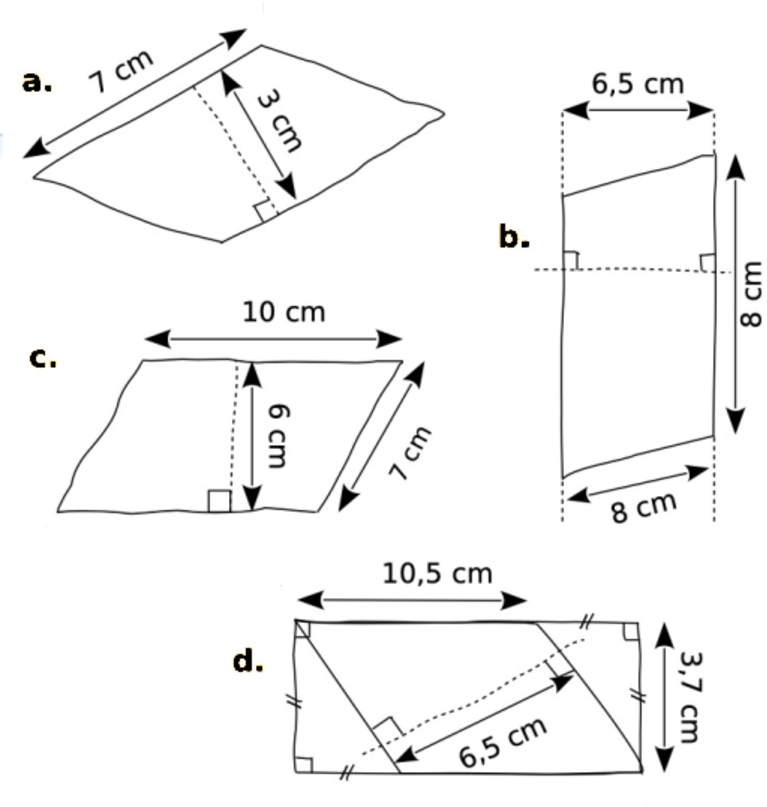
\includegraphics[width=7.9cm]{parallelogrammes}
         \end{center}
      \end{exercice}
      
      \begin{Solution}
         \begin{enumerate}
            \item $\mathcal{A}_a =\Lg{7}\times\Lg{3} =\cor{\Aire{21}}$.
            \item $\mathcal{A}_b =\Lg{8}\times\Lg{6,5} =\cor{\Aire{52}}$.
            \item $\mathcal{A}_c =\Lg{10}\times\Lg{6} =\cor{\Aire{60}}$.
            \item $\mathcal{A}_d =\Lg{10,5}\times\Lg{3,7} =\cor{\Aire{38,85}}$.
         \end{enumerate}
      \end{Solution}
      
      
      \begin{exercice} %5
         Déterminer la longueur inconnue.
         \begin{enumerate}
            \item Parallélogramme de base \Lg{8} et d'aire \Aire{24}. \par
               Calculer la hauteur.
            \item Parallélogramme de hauteur \Lg{30} et d'aire \Aire[dm]{2,1}. \par
               Calculer la mesure de la base relative à cette hauteur.
         \end{enumerate}
      \end{exercice}
      
      \begin{Solution}
         \begin{enumerate}
            \item $\mathcal{A} =\Lg{8}\times h =\Aire{24}$ soit $h =\dfrac{\Aire{24}}{\Lg{8}} =\Lg{3}$. \par \smallskip
               La \cor{hauteur} du parallélogramme mesure \cor{\Lg{3}}. \smallskip
            \item $\mathcal{A} =b\times\Lg{30} =\Aire{210}$ ; $b =\dfrac{\Aire{210}}{\Lg{30}} =\Lg{7}$. \par \smallskip
               La \cor{base} du parallélogramme mesure \cor{7 cm}.
         \end{enumerate}
      \end{Solution}
      
      
      \begin{exercice} %6
         Un menuisier doit découper une planche selon le plan suivant :
         \begin{center}
            {\psset{unit=0.7} \footnotesize
            \begin{pspicture}(0,-0.5)(8,4.5)
               \pspolygon(0,0)(5,0)(8,1)(8,4.5)(5,3.5)(0,3.5)
               \psline(5,0)(5,3.5)
               \psline{<->}(0,-0.3)(8,-0.3)
               \rput(4,-0.7){\Lg{80}}
               \psline{<->}(-0.3,0)(-0.3,3.5)
               \rput{90}(-0.7,1.75){\Lg{35}}
               \psline{<->}(0,3.8)(5,3.8)
               \rput(2.5,4.2){\Lg{50}}
            \end{pspicture}}
         \end{center}
         \begin{enumerate}
            \item Calculer l'aire de la planche.
            \item Le menuisier doit faire deux ouvertures dans cette planche :
               \begin{itemize}
                  \item une ouverture rectangulaire de \Lg{40} sur \Lg{15} ;
                  \item une ouverture en parallélogramme de base \Lg{20} et de hauteur \Lg{13}.
               \end{itemize}
            Calculer la nouvelle aire de la planche.
         \end{enumerate}
      \end{exercice}
      
      \begin{Solution}
         \begin{enumerate}
            \item Aire de la planche de gauche : \par
            $\mathcal{A}_1 =\Lg{50}\times\Lg{35} =\Aire{1750}$. \par
               Aire de la planche de droite : \par
               $\mathcal{A}_2 =\Lg{35}\times(\Lg{80}-\Lg{50}) =\Lg{35}\times\Lg{30}$ \par
               $=\Aire{1050}$. \par
               Aire de la planche complète : \par
               $\mathcal{A}_1+\mathcal{A}_2 =\Aire{1750}+\Aire{1050} =\Aire{2800}$. \par
               L'aire de la planche est de \cor{\Aire{2800}}.
            \item Ouverture rectangulaire : \par
               $\mathcal{A}_3 =\Lg{40}\times\Lg{15} =\Aire{600}$. \par
               Ouverture du parallélogramme : \par
               $\mathcal{A}_4 =\Lg{20}\times\Lg{13} =\Aire{260}$. \par
               $\mathcal{A}_3+\mathcal{A}_4 =\Aire{600}+\Aire{260} =\Aire{860}$. \par
               La nouvelle aire de la planche est de \par
               $\Aire{2800}-\Aire{860} =\cor{\Aire{1940}}$.
         \end{enumerate}
      \end{Solution}

   \end{multicols}

\end{Maquette}


%%% Récré %%%
\begin{Maquette}[Cours]{Theme={Activité récréative},Couleur={IndianRed}}
    
   \ARtitre{La formule de Pick}
      
      On travaille dans un réseau pointé à maille carrée. On note $u.\ell.$ l'unité de longueur et $u.a.$ l'unité d'aire. \par
      On appelle polygone de Pick, un polygone non aplati construit sur un tel réseau et dont chacun des sommets est un point du réseau. On considère les figures $FORMULE$ et $PICK$ suivantes :
      \begin{center}  
         {\psset{unit=0.5}\small
         \begin{pspicture}(6,0)(28,11.5)
            \pstGeonode[fillstyle=solid,fillcolor=lightgray!30,CurveType=polygon,PosAngle={45,135,-135,-50,-30,45}](9,10){R}(7,6){O}(7,1){F}(12,1){E}(16,3){L}(16,6){U}(12,6){M}
            \psframe[fillstyle=solid,fillcolor=lightgray!30](22,9)(23,10)
            \pstGeonode[fillstyle=solid,fillcolor=lightgray!30,CurveType=polygon,PosAngle={-150,-45,30,135}](18,1){P}(24,1){I}(27,5){C}(21,5){K}
            \psgrid[griddots=1,gridlabels=0,subgriddiv=1,gridwidth=0.5mm](6,0)(28,11)
            \rput(22.5,8.5){1 $u.a.$}
            \psline{<->}(18,9)(19,9)
            \rput(18.5,8.5){1 $u.\ell.$}      
         \end{pspicture}}
      \end{center}
      
      \ARpartie{Avec les formules classiques}
         \begin{enumerate}
            \item Calculer l'aire du parallélogramme $PICK$ en unité d'aire. \par \medskip
               \pointilles 
            \item Calculer l'aire du polygone $FORMULE$, en unité d'aire en détaillant les étapes du raisonnement. \par \medskip
               \pointilles  \par \medskip
               \pointilles \smallskip
         \end{enumerate}
      
      \ARpartie{avec la formule de Pick}
         La formule de Pick permet de calculer l'aire $\mathcal{A}$ d'un polygone de Pick, à partir du nombre $i$ de points du réseau strictement intérieurs à ce polygone et du nombre $b$ de points du réseau sur le bord du polygone : \fbox{$\mathcal{A} =i+\dfrac{b}{2}-1$}. 
         \begin{enumerate}
         \setcounter{enumi}{2}
            \item Appliquer cette formule au parallélogramme $PICK$. \par \bigskip
               $i =\pointilles  \quad b =\pointilles $ \quad donc, $\mathcal{A} = \pointilles $ \par
            \item Appliquer cette formule au polygone $FORMULE$. \par \bigskip
               $i =\pointilles  \quad b =\pointilles $ \quad donc, $\mathcal{A} = \pointilles $ \par
            \item Appliquer la formule de Pick aux trois polygones de Pick $MOFE$, $MOR$ et $MULE$. \par
               Vérifier que la somme des résultats obtenus est égale à l'aire totale de la figure. \par \medskip
               \pointilles \par \medskip
               \pointilles \par \medskip
               \pointilles 
         \end{enumerate}

\end{Maquette}